\subsubsection{Using lazy expression syntax for if-else-statements in function expressions}
\label{sec:lazy-expression}
\textit{This section was contributed by Magali Billen}\\
This cookbook provides an example to illustrate how to use the lazy-expression syntax for multiple, nested, if-else-statements in function expressions in the parameter file. It also shows how to set parameters in the input file so you can quickly check initial conditions (i.e., without waiting for the solver to converge).  For this model we define a simple 2D box, which is $5000 \times 1000$ km, with free-slip velocity boundary conditions. The material parameters are constant within the box (set using the  ``simple'' material model). The initial thermal structure has two parts divided at $xtr=2200$~km. The temperature in each region is defined using the equation for a half-space cooling model:
\begin{equation}
T(x,y) = T_s + (T_m  - T_s) \erf{(\frac{y}{2\sqrt{\kappa x/v}})}
\end{equation}
where $\erf$ is the error function, $T_m$ is the mantle temperature, $T_s$ is the surface temperature, $y$ is depth, $x$ is horizontal distance, $\kappa$ is the thermal diffusivity, and $v$ is the plate velocity. The age of the plate is given by $x/v$. Note that the equation for the half-space cooling model is not defined at $x=0$ (because there is a divide by zero inside the error function): at $x=0$, $T=T_m$.  For $(x \le xtr)$ and $(x>0)$ the age of the plate increases from zero at the boundary according to a fixed plate velocity $v_\text{sub}=7.927\times10^{-10}$~m/s  ($2.5$~cm/yr). This is the subducting plate. For $x > xtr$, there is a fixed plate age of $age_{op}=9.46\times10^{14}$~s ($30$~my); this is the overriding plate. In order to resolve the temperature structure, we also define some initial refinement of the mesh for the top 150 km of the mesh. Both the mesh refinement and the temperature structure are defined using lazy-expression syntax in functions within the parameter file.

Functions can be used in the parameter file to define initial conditions (e.g., temperature, composition), boundary conditions, and even to set regions of refinement. We also often want to use different values of functions in different regions of the model (e.g., for the two plates as described above) and so we need to use if-statements to specify these regions. The function constants and expressions are read in using the muparser. The muparser accepts two different syntax options for if-statements (see also Section \ref{sec:muparser-format}).
\begin{enumerate}
\item \texttt{if(condition, true-expression, false-expression)}
\item \texttt{(if-condition ?\ true-expression :\ false-expression)}  \textbf{lazy-expression syntax}
\end{enumerate}
In the first syntax, both the true and false expression are evaluated (even though only one is needed), while in the second  syntax, only the expression that is needed for the prescribed if condition is evaluated. In the lazy expression the \texttt{?} represents the ``then'', and the \texttt{:} represents the ``else'' in the if-then-else statement. Because the function expression is evaluated for every mesh point, for the plate temperature described above, it is necessary to use the lazy expression syntax to avoid evaluating the full temperature equation at mesh points where $x=0$ because this will create a floating-point exception.  The function expression shown in the snippet from the parameter file below uses nested if-else-statements with this structure:\\
\texttt{if ((x>0.0) \&\& (x<=xtr))  then T-sub else (if (x>xtr) then T-ov else Tm)}\\
where T-sub is the function for the temperature of the subducting plate and T-ov is the function for the temperature of the
overriding plate.
\lstinputlisting[language=prmfile]{temperature.part.prm.out}
Notice also that the boundary conditions for the temperature are defined in a separate subsection and depend on the geometry.
The boundary conditions are insulating (zero flux) side-walls and fixed temperature at the top and bottom. Figure \ref{lazy-expression-tempic} shows the initial temperature on the full domain.
\begin{figure}
\centering
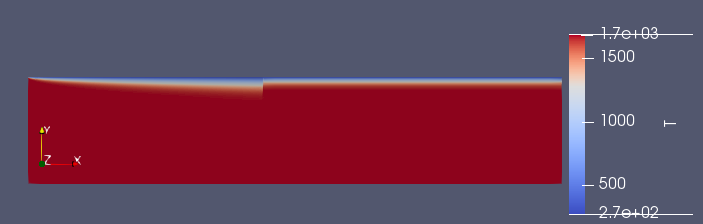
\includegraphics[width=0.8\textwidth]{initial_temperature.png}
\caption{\it Initial temperature condition for the lazy-expression syntax cookbook. \label{lazy-expression-tempic}}
\end{figure}

The structure and refinement of the mesh are determined in two subsections of the parameter file. First, because the model domain is not a square, it is necessary to subdivide the domain into sections that are equidimensional (or as close as possible): this is done using the \texttt{repetitions} parameters in the \texttt{Geometry} section. In this case because the model domain has an aspect ratio of 5:1, we use 5 repetitions in the $x$ direction, dividing the domain into 5 equidimensional elements each 1000 by 1000 \si{km}.
\lstinputlisting[language=prmfile]{repetitions.part.prm.out}
Further refinements will divide each sub-region multiple times keeping the aspect ratio of the sub-region. In this case, we refine the elements in each subregion 3 more times. We then use the \texttt{minimum refinement function} strategy and use the \texttt{if-then-else} statement in the function expression to refine 4 more times to a refinement level of 7, but only where the depth is less than \SI{150}{km}. Appropriate values of the minimum refinement level in this function expression could be the sum of initial global refinement level (3) and initial adaptive refinement level (4) in the `\texttt{then}' statement (i.e., 7 here) and the value of initial global refinement in the `\texttt{else}' statement.
\lstinputlisting[language=prmfile]{mesh-refinement.part.prm.out}
Figure \ref{lazy-expression-tempic-zoom} zooms in on the region where the two plates meet and shows the temperature on a wireframe highlighting the element size refinement. Notice that the mesh refinement algorithm automatically adjusts the element size between the region that is specific to be a level 7 and the region at level 3 to create a smooth transition in element size.
\begin{figure}
\centering
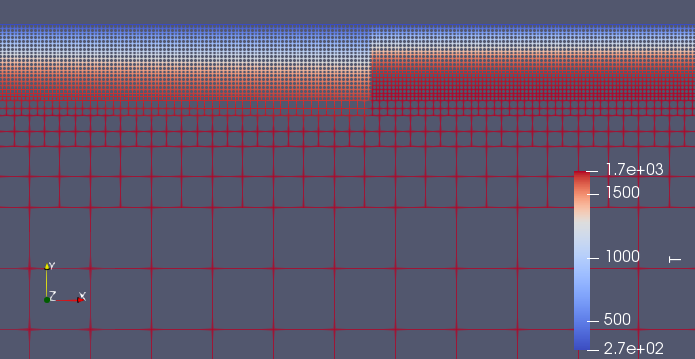
\includegraphics[width=0.5\textwidth]{initial_temperature_on_mesh_zoom.png}
\caption{\it Initial temperature condition for the lazy-expression syntax cookbook within the region where the two plates meet. The wireframe shows the element size refinement. \label{lazy-expression-tempic-zoom}}
\end{figure}

Finally, in order to just test whether the initial temperature structure has been properly defined, it is helpful to run the model for a single time-step and without actually waiting for the solvers to converge. In order to do this, the \texttt{End time} can be set to zero. If the model is very large (lots of refinement) or there are large viscosity jumps that take longer to converge in the Stokes solver, it can also be useful to set the solver tolerance parameters to large values as noted below. However, remember that in that case the solution will not be converged -- it is only useful for checking that the initial condition is set correctly.
\lstinputlisting[language=prmfile]{check-initial-condition.part.prm.out}


